\section{Introduction}

Accurate 3D hand and human pose estimation is an important requirement for activity recognition with diverse applications, such as human-computer interaction or augmented reality~\cite{romero2009monocular}. It has been studied for decades in computer vision community and has attracted considerable research interest again due to the introduction of low-cost depth cameras.

\begin{figure}[t]
\begin{center}
   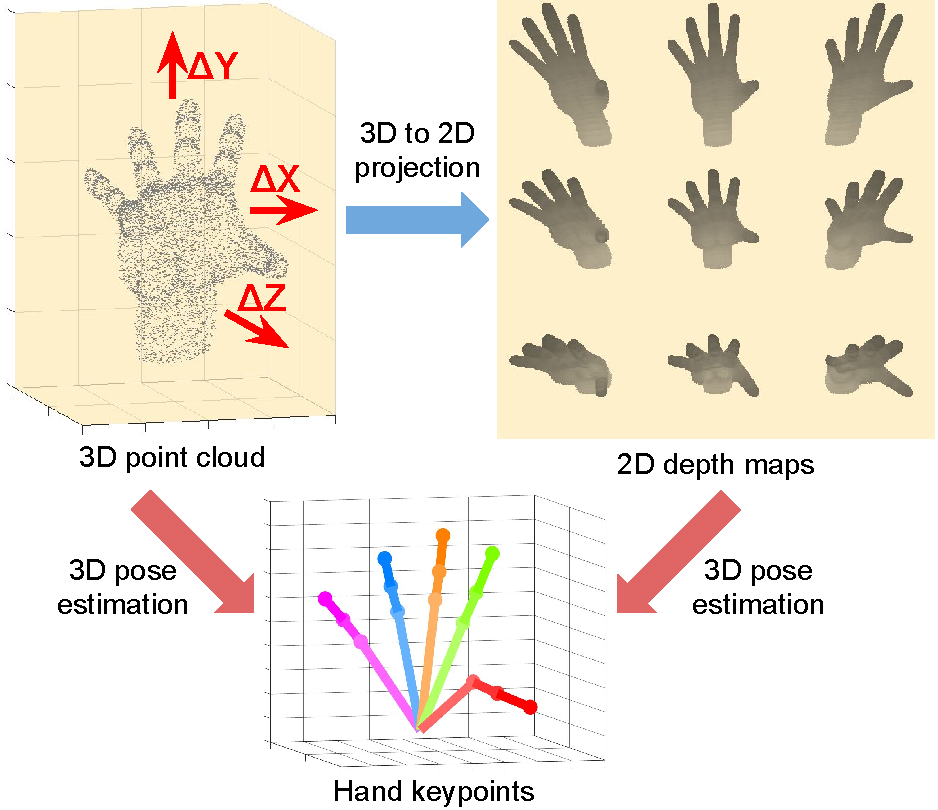
\includegraphics[width=1.0\linewidth]{weakness_of_prev.pdf}
\end{center}
\vspace*{-5mm}
   \caption{Visualization of perspective distortion in 2D depth image. The 3D point cloud has one-to-one relation with a 3D pose, but the 2D depth image has many-to-one relation because of perspective distortion. Thus, the network is compelled to perform perspective distortion-invariant estimation. The 2D depth maps are generated by translating the 3D point cloud by $\Delta$X = -300, 0, 300 mm (from left to right) and $\Delta$Y = -300, 0, 300 mm (from bottom to top). In all cases, $\Delta$Z is set to 0 mm. Similar values to the real human hand size and camera projection parameters in the MSRA dataset were used for our visualization.}
\vspace*{-3mm}
\label{fig:weakness_of_prev}
\end{figure}

Recently, powerful discriminative approaches based on convolutional neural networks (CNNs) are outperforming existing methods in various computer vision tasks including 3D hand and human pose estimation from a single depth map~\cite{ge20173d,guo2017towards,Oberweger_2017_ICCV_Workshops,chen2017pose,haque2016towards}. Although these approaches achieved significant advancement in 3D hand and human pose estimation, they still suffer from inaccurate estimation because of severe self-occlusions, highly articulated shapes of target objects, and low quality of depth images. Analyzing previous deep learning-based methods for 3D hand and human pose estimation from a single depth image, most of these methods~\cite{oberweger2015hands,oberweger2015training,bouchacourt2016disco,Wan_2017_CVPR,guo2017ren,guo2017towards,Oberweger_2017_ICCV_Workshops,chen2017pose,madadi2017end,fourure2017multi,haque2016towards} are based on a common framework that takes a 2D depth image and directly regresses the 3D coordinates of keypoints, such as hand or human body joints. However, we argue that this approach has two serious drawbacks. The first one is perspective distortion in 2D depth image. As the pixel values of a 2D depth map represent the physical distances of object points from the depth camera, the depth map is intrinsically 3D data. However, most previous methods simply take depth maps as a 2D image form, which can distort the shape of an actual object in the 3D space by projecting it to the 2D image space. Hence, the network \emph{see} a distorted object and is burdened to perform distortion-invariant estimation. We visualize the perspective distortions of the 2D depth image in Figure~\ref{fig:weakness_of_prev}. The second weakness is the highly non-linear mapping between the depth map and 3D coordinates. This highly non-linear mapping hampers the learning procedure and prevents the network from precisely estimating the coordinates of keypoints as argued by Tompson \etal~\cite{tompson2014joint}. This high nonlinearity is attributed to the fact that only one 3D coordinate for each keypoint has to be regressed from the input.

To cope with these limitations, we propose the \emph{voxel-to-voxel prediction network for pose estimation (V2V-PoseNet)}. In contrast to most of the previous methods, the V2V-PoseNet takes a voxelized grid as input and estimates the per-voxel likelihood for each keypoint as shown in Figure~\ref{fig:comparison_io_type}. 

By converting the 2D depth image into a 3D voxelized form as input, our network can \emph{sees} the actual appearance of objects without perspective distortion. Also, estimating the per-voxel likelihood of each keypoint enables the network to learn the desired task more easily than the highly non-linear mapping that estimates 3D coordinates directly from the input. We perform a thorough experiment to demonstrate the usefulness of the proposed volumetric representation of input and output in 3D hand and human pose estimation from a single depth map. The performance of the four combinations of input (i.e., 2D depth map and voxelized grid) and output (i.e., 3D coordinates and per-voxel likelihood) types are compared.

The experimental results show that the proposed voxel-to-voxel prediction allows our method to achieve the state-of-the-art performance in almost all of the publicly available datasets (i.e., three 3D hand~\cite{tompson2014real,tang2014latent,sun2015cascaded} and one 3D human~\cite{haque2016towards} pose estimation datasets) while it runs in real-time. We also placed first in the HANDS 2017 frame-based 3D hand pose estimation challenge~\cite{yuan20172017}. We hope that the proposed system to become a milestone of 3D hand and human pose estimation problems from a single depth map. Now, we assume that the term \enquote{3D pose estimation} refers to the localization of the hand or human body keypoints in 3D space.

Our contributions can be summarized as follows. 
\begin{itemize}
\item We firstly cast the problem of estimating 3D pose from a single depth map into a voxel-to-voxel prediction. Unlike most of the previous methods that regress 3D coordinates directly from the 2D depth image, our proposed V2V-PoseNet estimates the per-voxel likelihood from a voxelized grid input. 

\item We empirically validate the usefulness of the volumetric input and output representations by comparing the performance of each input type (i.e., 2D depth map and voxelized grid) and output type (i.e., 3D coordinates and per-voxel likelihood).

\item We conduct extensive experiments using almost all of the existing 3D pose estimation datasets including three 3D hand and one 3D human pose estimation datasets. We show that the proposed method produces significantly more accurate results than the state-of-the-art methods. The proposed method also placed first in the HANDS 2017 frame-based 3D hand pose estimation challenge.
\end{itemize}
